\label{sec:evaluation}

We evaluate \doubletake{} on a quiescent Intel Core 2 dual-processor system with 16GB of RAM running Linux 2.6.18-194.17.1.el5, and version 2.5 of \texttt{glibc}. Each processor is a 4-core 64-bit Intel Xeon, operating at 2.33GHz with a 4MB shared L2 cache a 32KB per-core L1 cache. All benchmarks are built as 64-bit executables using LLVM 3.2 with the clang front-end and \texttt{-O2} optimizations.

Our evaluation measure the runtime and memory overhead of \doubletake{}, and the effectiveness of the heap buffer overflow, memory leak, and use-after-free detectors.

\subsection{Performance Overhead}
\label{sec:perf}

\begin{figure*}[!ht]
	\begin{center}
		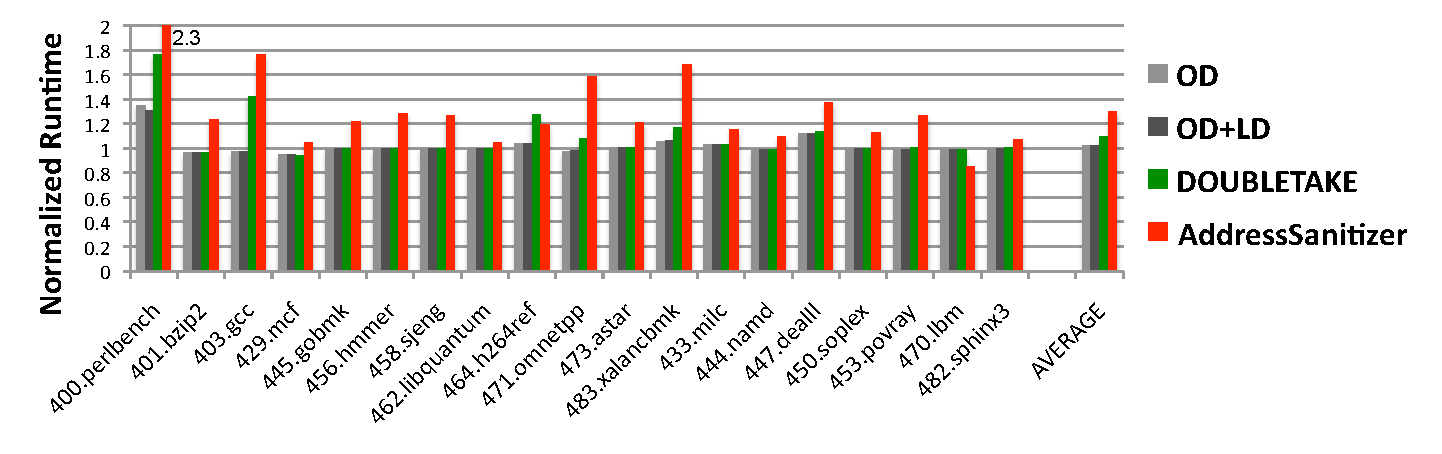
\includegraphics[width=6.5in]{doubletake/figure/perf}
	\end{center}
	\caption{This figure shows the runtime overhead of \doubletake{} (OD - Buffer Overflow Detection, LD - Leak Detection, \doubletake{} - with three detections enabled) and AddressSanitizer, normalized to each benchmark's original execution time. 
%Overhead for Valgrind is reported in Table~\ref{table:valgrind} because the results do not fit on this graph.
\label{fig:perf}}
\end{figure*}

\begin{table}[t]
	\centering
	\begin{tabular}{r|c p{0.1em} r|c}
		\textbf{Benchmark} & \textbf{Overhead} & & \textbf{Benchmark} & \textbf{Overhead} \\
		\cline{1-2} \cline{4-5}
		400.perlbench	& 20.5X	& & 458.sjeng	& 20.3X	\\
		401.bzip2		& 16.8X	& & 471.omnetpp	& 13.9X	\\
		403.gcc			& 18.7X	& & 473.astar	& 11.9X	\\
		429.mcf			& 4.5X 	& & 433.milc		& 11.0X	\\
		445.gobmk		& 28.9X	& & 444.namd		& 24.9X	\\
		456.hmmer		& 13.8X	& & 450.dealII	& 42.8X	\\
	\end{tabular}
	\caption{Valgrind's runtime overhead. \label{table:valgrind}}
\end{table}


We evaluate performance on all C and C++ SPEC CPU2006 benchmarks, 19 applications in total. We compare \doubletake{} with AddressSanitizer and Valgrind. AddressSanitizer is the previous state-of-the-art for detecting buffer overflows and use-after-free errors~\cite{AddressSanitizer}, but cannot detect memory leaks. Valgrind's Memcheck tool is widely used tool to detect buffer overflows, memory leaks, and use-after-free errors~\cite{overflow:valgrind}. 

During performance evaluation, we disable \doubletake{}'s rollback functionality to only measure the overhead of normal execution. \doubletake{} only detects memory errors of the heap, thus AddressSanitizer is run without checks on accesses to the stack and globals, and without checks on read accesses. For each benchmark, we report the average of three runs with the largest input size, except for Valgrind. We only run Valgrind once because of its slowness. 

Performance results of \doubletake{} and AddressSanitizer are shown in Figure~\ref{fig:perf}. Results for Valgrind do not fit on the graph, and are presented separately in Table~\ref{table:valgrind}. On average, \doubletake{} adds only $9\%$ overhead \emph{with all three error detectors enabled}. If \doubletake{} do not detect memory use-after-free errors, the performance overhead is under 3\% on average. AddressSanitizer slows execution by $30\%$ on average, and Valgrind has an average overhead of $19X$ on all evaluated benchmarks. Because Valgrind is running too slow, we haven't finished the evaluation on all benchmarks. Also, we kill a program if it is already running $20\times$ slower, including \texttt{400.perlbench} and \texttt{458.sjeng}. 

% difference across all different tools
For 17 out of 19 benchmarks, \doubletake{} outperforms AddressSanitizer, even with an additional memory leak detection. For 12 benchmarks, \doubletake{}'s runtime overhead is under 3\%. \doubletake{} substantially outperforms Valgrind for all benchmarks. For both \doubletake{} and AddressSanitizer,  \texttt{400.perlbench}, \texttt{403.gcc} and \texttt{447.deallIII} benchmark introduce much more performance overhead than other benchmarks. We also observe that they all introduce much more memory overhead (in terms of absolute value), according our experimental results in Table~\ref{tbl:memoryoverhead}. These significant memory overhead may reduce the ratio of cache efficiency, thus causing performance problem. 



% Difference across all different tools
From the figure, we also notice that detection of memory use-after-free adds about 6\% performance overhead averagely, although most of overhead are coming from \texttt{400.perlbench}, \texttt{403.gcc} and \texttt{464.h264ref} benchmark. As described in Section~\ref{sec:danglingpointer}, \doubletake{} has to fill every freed object up to 128 bytes with canaries and check those canaries when a freed object is released to the program heap. If an application has a big number of memory allocation and de-allocation, these operations consist of most of performance overhead. 




Table 3 shows detailed benchmark characteristics. The “Processes” column shows the number of different invocations in the input set. The number of epochs is significantly lower than the number of system calls because of \doubletake{}'s lightweight system call handling. Benchmarks with the highest overhead run a substantial number of epochs (perlbench and h264ref) and make a large number of malloc calls (gcc, omnetpp, and
xalancbmk).



\subsection{Memory Overhead}
\label{sec:memoverhead}

\begin{table}[t]
\centering
\begin{tabular}{l|c|c|c|}
\textbf{ \small Benchmark} & \textbf{\small Original} &  \textbf{\small AddressSanitizer} & \textbf{\small \doubletake{} } \\
\hline
400.perlbench & 656 &	1481 & 1977 \\
401.bzip2	& 870 &	1020 &	1003 \\
403.gcc	& 683 &	2293 &	1583 \\
429.mcf	& 1716 &	1951 &	1994 \\
445.gobmk &	28 &	137 &	58 \\
456.hmmer &	24 &	256 &	129 \\
458.sjeng & 179 & 220 &	203 \\
462.libquantum	& 66 &	144 &	131 \\
464.h264ref	& 65 &	179 &	247 \\
471.omnetpp	& 172 &	538 &	291 \\
473.astar	& 333 &	923 &	477 \\
483.xalancbmk &	428 & 1149 &	801 \\
433.milc	& 695 &	1008 &	917 \\
444.namd	& 46 &	79 &	92 \\
447.dealII	& 514 &	2496 &	1727 \\
450.soplex	& 441 &	1991 &	1654 \\
453.povray	& 3 &	133 &	50 \\
470.lbm	& 418 &	496 &	470 \\
482.sphinx3 &	45 &	181 & 98 \\
\hline
Total & 7386 & 16678 & 13906 \\
\hline
\end{tabular}
\caption{Memory Usage of \doubletake{} and AddressSanitizer(MB).\label{tbl:memoryoverhead}}
\end{table}


\begin{figure*}
\begin{center}
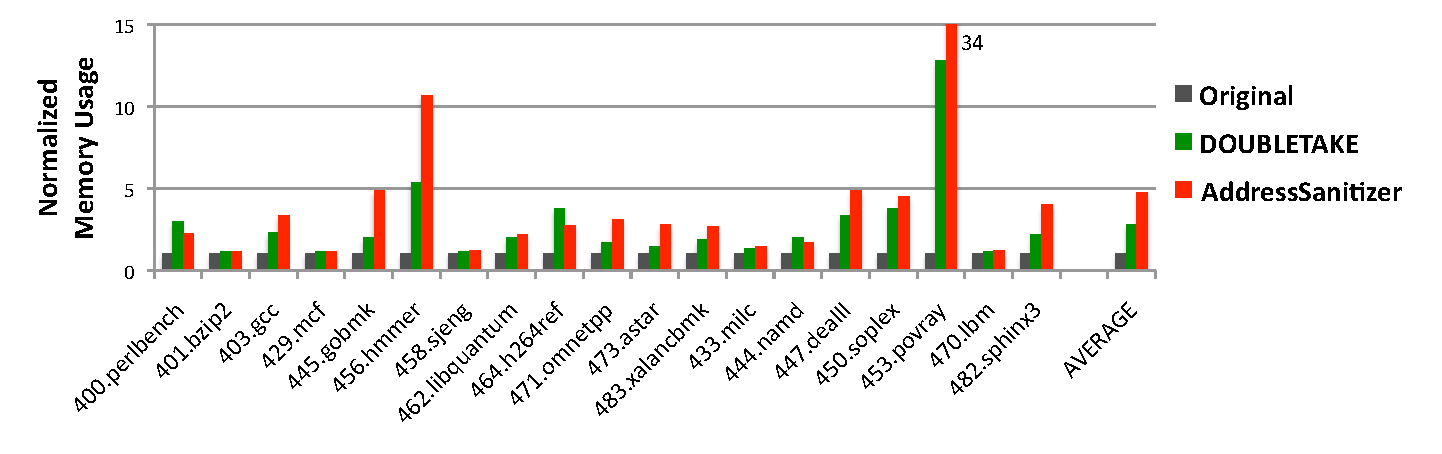
\includegraphics[width=6.5in]{doubletake/figure/memory}
\end{center}
\caption{
Memory overhead of \doubletake{} and AddressSanitizer.
\label{fig:memory}}
\end{figure*}

Memory overhead of \doubletake{} comes from the following aspects. Firstly, snapshot in the beginning of each epoch, by backing up the globals, the heap and the stack, contributes the most significant memory overhead of \doubletake{}. Snapshot can double the memory usage. However, the first snapshot happening in the beginning of a program normally doesn't take too much memory since there is no heap usage at all. Thus, this explains why \texttt{401.bzip2}, \texttt{429.mcf}, \texttt{458.sjeng},  \texttt{433.milc}, and \texttt{470.lbm} have less than $2\times$ memory overhead. Secondly, recording results of system calls introduce some memory overhead. Additionally, different applications may introduce different memory overhead. For the detection of heap buffer overflows and memory leakage, \doubletake{} adds canaries around each heap object and maintains a bit map to indicate canary locations. For the detection of memory usage-after-free errors, \doubletake{} delays memory re-usage by putting freed objects into a quarantine list, which also introduces constant additional memory overhead. 

We only evaluate the physical memory overhead here because \doubletake{} pre-allocates a huge block of heap, which is 4GB virtual memory and should not be counted as memory overhead. Also, we all only care about physical memory overhead when virtual memory overhead is practically infinite in 64bit machine. Proportional set size (PSS) in \texttt{/proc/self/smaps} reflects physical memory increase on the existing system by running an application. Thus, we periodically collect this data and use the sum of different memory mappings as total physical memory usage. We presents the normalized memory overhead of running different benchmarks in Figure~\ref{fig:memory}. We also list the actual memory usage of \doubletake{} and AddressSanitizer in Table~\ref{tbl:memoryoverhead}.

From Figure~\ref{fig:memory}, \doubletake{}'s memory overhead is 2.8$\times$, while AddressSanitizer's overhead is 4.8$\times$. For \texttt{453.povray} and \texttt{464.h264ref}, both AddressSanitizer and \doubletake{} has very high normalized memory overhead because the original memory usage of this benchmark is extremely low, only 3 and 24 megabytes. But for other benchmarks, both AddressSanitizer and \doubletake{} has memory overhead lesss than $5\times$. For all benchmarks except \texttt{400.perlbench} and \texttt{444.namd}, \doubletake{} has lower memory overhead. 
From Table~\ref{tbl:memoryoverhead}, AddressSanitizer totally spends about 20\% more memory than \doubletake{}. In total, \doubletake{} memory overhead is less than 2$\times$ of original memory usage. 

\subsection{Effectiveness}
\label{sec:effect}


We use \doubletake{} to find errors in both the SPEC CPU2006
benchmark suite and a suite of real applications.

\emph{Benchmarks.} During the evaluation of SPEC CPU2006 benchmarks, \doubletake{} detected a one-byte heap buffer overflow
 in \texttt{perlbench}, which can not be detected by AddressSanitizer. \doubletake{} also detected a big number of memory leaks in \texttt{perlbench} and \texttt{gcc}, which has been verified using Valrind.

\emph{Real Applications.} For buffer overflows, we have evaluated the effectiveness on  six real applications. \texttt{libHX} has been evaluated in previous work~\cite{overflow:Cruiser}. \texttt{bzip2}~\cite{bzip2overflow} and \texttt{vim} ~\cite{vimoverflow} are got from Red Hat Bugzilla. Other benchmarks are from bugbench~\cite{bugbench}. We especially turn global array buffer overflow in \texttt{bzip2}, \texttt{gzip}, and \texttt{polymorphy} to heap buffer overflows. \doubletake{} successfully caught all these found heap buffer overflows. The buffer overflows we observed in these applications are triggered by specific inputs, which are difficult to detect during development. \doubletake{}'s overhead is low enough to be enabled in deployment, which would make it possible to detect these bugs in the field.
\doubletake{} also detects memory leaks in \texttt{gcc-4.4.7} and \texttt{vim}.